% TODO - Key Idea Slide
% Combine Vulkan and CUDA to run a 
% tightly-coupled in-situ visualization 
% at interactive speeds in real-time.
\begin{frame}
    \frametitle{Project Goal}
\begin{center}
    
% \begin{tikzpicture}[
% textnode/.style={text width=10cm},
% ]
%     \node[textnode] at (0,0) {\Large Create a \emph{tightly-coupled in-situ} visualization};
%     \node[textnode] at (0.5,-1) {\Large with \emph{Vulkan \& CUDA}};
%     \node[textnode] at (0.5,-2) {\Large that runs at \emph{interactive speeds} in \emph{real-time}.};
% \end{tikzpicture}

{\LARGE Create a {tightly-coupled in-situ} visualization
with {Vulkan \& CUDA}\vspace{1em}
that runs at {interactive speeds} in {real-time}.}

\vspace{1in}

This is very verbose - let's break it down.

\end{center}
\end{frame}

\begin{frame}
    \frametitle{Project Goal}
    \framesubtitle{Let's clarify!}

\begin{tikzpicture}[
textnode/.style={align=left, anchor=west},%text width=10cm},
overlaynode/.style={anchor=east,align=right,red},
]
    \node[textnode](a) at (0,0) {\LARGE Create a \textbf{tightly-coupled in-situ} visualization} ;
    \node[textnode](b) at (0.5,-1.5) {\LARGE with \textbf{Vulkan \& CUDA}} ;
    \node[textnode](c) at (0.5,-3) {\LARGE that runs at \textbf{interactive speeds} in \textbf{real-time}.} ;
\end{tikzpicture}
\end{frame}

% TODO - Breakdown #1
% Vulkan/CUDA
\begin{frame}
    \frametitle{Project Goal}
    \framesubtitle{Let's clarify!}

\begin{tikzpicture}[
textnode/.style={align=left, anchor=west},%text width=10cm},
overlaynode/.style={anchor=east,align=right,red},
]
    \node[textnode](a) at (0,0) {\LARGE Create a \textbf{tightly-coupled in-situ} visualization} ;
    \node[textnode](b) at (0.5,-1.5) {\LARGE with \textbf{Vulkan \& CUDA}} ;
    \node[textnode](c) at (0.5,-3) {\LARGE that runs at \textbf{interactive speeds} in \textbf{real-time}.} ;
    
    \begin{scope}[overlay]
    \node[overlaynode](a_h) at (14,0.5) {Simulate and Visualize at the same time,\\on the same machine\todocite{}};
    
    % \node[overlaynode](b_h) at (12,-1.5) {Rendering and Compute APIs for GPUs};

    % \node[overlaynode, anchor=south](c_h1) at (5,-3.2) {Update 60 times per second};
    % \node[overlaynode, anchor=north](c_h2) at (10,-4.8) {Should simulate at the same speed as real life};

    \draw[red] (a.north) -- (a_h.west);
    % \draw[red] (b.east) -- (b_h.west);
    % \draw[red] (c.north) -- (c_h1.south);
    % \draw[red] (c.east) -- (c_h2.north);
    \end{scope}
\end{tikzpicture}
\end{frame}

% TODO - Breakdown #2
% in-situ, tightly-coupled
\begin{frame}
    \frametitle{Project Goal}
    \framesubtitle{Let's clarify!}

\begin{tikzpicture}[
textnode/.style={align=left, anchor=west},%text width=10cm},
overlaynode/.style={anchor=east,align=right,red},
]
    \node[textnode](a) at (0,0) {\LARGE Create a \textbf{tightly-coupled in-situ} visualization} ;
    \node[textnode](b) at (0.5,-1.5) {\LARGE with \textbf{Vulkan \& CUDA}} ;
    \node[textnode](c) at (0.5,-3) {\LARGE that runs at \textbf{interactive speeds} in \textbf{real-time}.} ;
    
    \begin{scope}[overlay]
    \node[overlaynode](a_h) at (14,0.5) {Simulate and Visualize at the same time,\\on the same machine\todocite{}};
    
    \node[overlaynode](b_h) at (12,-1.5) {Rendering and Compute APIs for GPUs};

    % \node[overlaynode, anchor=south](c_h1) at (5,-3.2) {Update 60 times per second};
    % \node[overlaynode, anchor=north](c_h2) at (10,-4.8) {Should simulate at the same speed as real life};

    \draw[red] (a.north) -- (a_h.west);
    \draw[red] (b.east) -- (b_h.west);
    % \draw[red] (c.north) -- (c_h1.south);
    % \draw[red] (c.east) -- (c_h2.north);
    \end{scope}
\end{tikzpicture}
\end{frame}

% TODO - Breakdown #3
% interactive speeds, real-time
\begin{frame}
    \frametitle{Project Goal}
    \framesubtitle{Let's clarify!}

\begin{tikzpicture}[
textnode/.style={align=left, anchor=west},%text width=10cm},
overlaynode/.style={anchor=east,align=right,red},
]
    \node[textnode](a) at (0,0) {\LARGE Create a \textbf{tightly-coupled in-situ} visualization} ;
    \node[textnode](b) at (0.5,-1.5) {\LARGE with \textbf{Vulkan \& CUDA}} ;
    \node[textnode](c) at (0.5,-4) {\LARGE that runs at \textbf{interactive speeds} in \textbf{real-time}.} ;
    
    \begin{scope}[overlay]
    \node[overlaynode](a_h) at (14,0.5) {Simulate and Visualize at the same time,\\on the same machine\todocite{}};
    
    \node[overlaynode](b_h) at (12,-1.5) {Rendering and Compute APIs for GPUs};

    \node[overlaynode, anchor=south](c_h1) at (5,-3.2) {Update 60 times per second};
    \node[overlaynode, anchor=north](c_h2) at (10,-4.8) {Should simulate at the same speed as real life};

    \draw[red] (a.north) -- (a_h.west);
    \draw[red] (b.east) -- (b_h.west);
    \draw[red] (c.north) -- (c_h1.south);
    \draw[red] (c.east) -- (c_h2.north);
    \end{scope}
\end{tikzpicture}
\end{frame}

% TODO - Overview slide
\begin{frame}{Overview}
    \todomark{Introduce Vulkan + CUDA}
\end{frame}